\documentclass[aspectratio=169,10pt]{beamer}
\usetheme{default}
\usepackage{booktabs}
\usepackage{graphicx}
\usepackage{amsmath,amssymb}
\usepackage{tikz}
\usepackage{array}
\usepackage{xcolor}
\usepackage{hyperref}
\usetikzlibrary{arrows.meta,positioning,fit}

\definecolor{ink}{HTML}{172033}
\definecolor{muted}{HTML}{64748B}
\definecolor{blue}{HTML}{2563EB}
\definecolor{orange}{HTML}{F97316}
\definecolor{green}{HTML}{16A34A}
\definecolor{red}{HTML}{DC2626}
\definecolor{pale}{HTML}{F1F5F9}
\setbeamercolor{normal text}{fg=ink,bg=white}
\setbeamercolor{frametitle}{fg=ink,bg=white}
\setbeamercolor{structure}{fg=blue}
\setbeamercolor{block title}{fg=white,bg=ink}
\setbeamercolor{block body}{fg=ink,bg=pale}
\setbeamertemplate{navigation symbols}{}
\setbeamertemplate{footline}{\hfill\color{muted}\insertframenumber\hspace{1em}\vspace{0.6em}}
\setbeamertemplate{frametitle}{\vspace{0.5em}\insertframetitle\par\vspace{-0.3em}\color{muted}\rule{\textwidth}{0.4pt}}
\setbeamersize{text margin left=0.65cm,text margin right=0.65cm}
\newcommand{\fig}[2]{\includegraphics[width=#1\textwidth]{#2}}
\newcommand{\good}[1]{\textcolor{green}{\textbf{#1}}}
\newcommand{\bad}[1]{\textcolor{red}{\textbf{#1}}}
\newcommand{\caveat}[1]{\textcolor{orange}{\textbf{#1}}}

\title{Spectral Gradient Filtering on Numerai}
\subtitle{From a broken comparison to a credible, bounded positive result}
\author{Titus Buckworth \quad Research record and audited experiment}
\date{14 August 2026}

\begin{document}

\begin{frame}[plain]
  \vfill
  {\fontsize{28}{32}\selectfont\bfseries\color{ink}Spectral Gradient Filtering\\on Numerai\par}
  \vspace{0.5em}
  {\Large\color{muted}What we tried, what went wrong, what eventually worked, and what remains unknown}
  \vspace{1.8em}
  \begin{columns}[T]
  \column{0.62\textwidth}
    \fig{1.0}{figures/outer-headline.png}
  \column{0.34\textwidth}
    \begin{block}{Audited bounded result}
      Spectral pipeline: \good{+0.00307 CORR}\\
      \good{3/3} random seeds win\\
      CORR Sharpe: \good{1.557 vs 1.265}
    \end{block}
    \vspace{0.4em}
    {\small\color{muted}This is evidence to continue, not yet a leaderboard claim.}
  \end{columns}
  \vfill
\end{frame}

\begin{frame}{Executive answer}
  \begin{columns}[T]
  \column{0.48\textwidth}
    \begin{block}{What finished}
      \begin{itemize}
        \item Corrected parameter-space spectral implementation
        \item Low- and high-rank exploratory studies
        \item Overparameterized 13.7M-parameter stress test
        \item Symmetric development selection on Numerai v5.3
        \item Frozen, chronological outer test and six-cell audit
      \end{itemize}
    \end{block}
  \column{0.48\textwidth}
    \begin{block}{What it means}
      \begin{itemize}
        \item \good{Serious competitor: yes}
        \item Spectral pipeline beat selected AdamW by 15.5\% relative CORR
        \item High-rank filtering strongly suppressed memorization
        \item \caveat{Not an optimizer-only causal comparison}
        \item \bad{Not yet leaderboard-comparable or submission-ready}
      \end{itemize}
    \end{block}
  \end{columns}
  \vspace{0.6em}
  \centering\large The next experiment should isolate the optimizer while extending the untouched time horizon.
\end{frame}

\begin{frame}{The motivating hypothesis}
  \begin{columns}[c]
  \column{0.55\textwidth}
  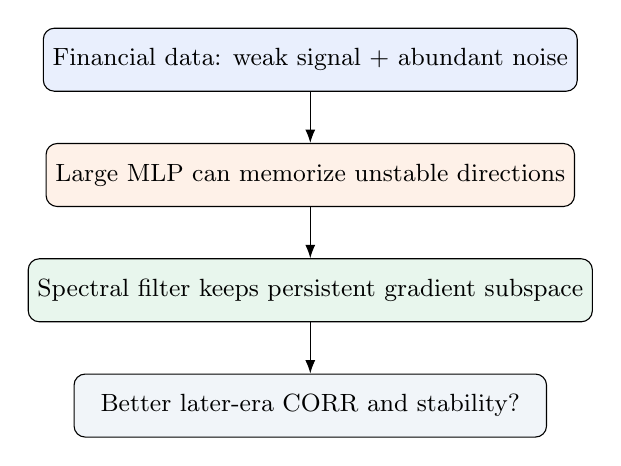
\begin{tikzpicture}[node distance=0.65cm, every node/.style={font=\small}]
    \node[draw,rounded corners,fill=blue!10,minimum width=6cm,minimum height=.8cm] (data) {Financial data: weak signal + abundant noise};
    \node[draw,rounded corners,fill=orange!10,below=of data,minimum width=6cm,minimum height=.8cm] (model) {Large MLP can memorize unstable directions};
    \node[draw,rounded corners,fill=green!10,below=of model,minimum width=6cm,minimum height=.8cm] (filter) {Spectral filter keeps persistent gradient subspace};
    \node[draw,rounded corners,fill=pale,below=of filter,minimum width=6cm,minimum height=.8cm] (goal) {Better later-era CORR and stability?};
    \draw[-{Latex}] (data)--(model); \draw[-{Latex}] (model)--(filter); \draw[-{Latex}] (filter)--(goal);
  \end{tikzpicture}
  \column{0.41\textwidth}
    \begin{block}{Why Numerai?}
      \begin{itemize}
        \item Extremely low signal-to-noise ratio
        \item Many anonymized candidate predictors
        \item Time and regime shift matter
        \item Exact per-era evaluation
        \item Public competitive benchmark
      \end{itemize}
    \end{block}
  \end{columns}
\end{frame}

\begin{frame}{What the dataset looks like}
  \begin{columns}[T]
  \column{0.52\textwidth}
    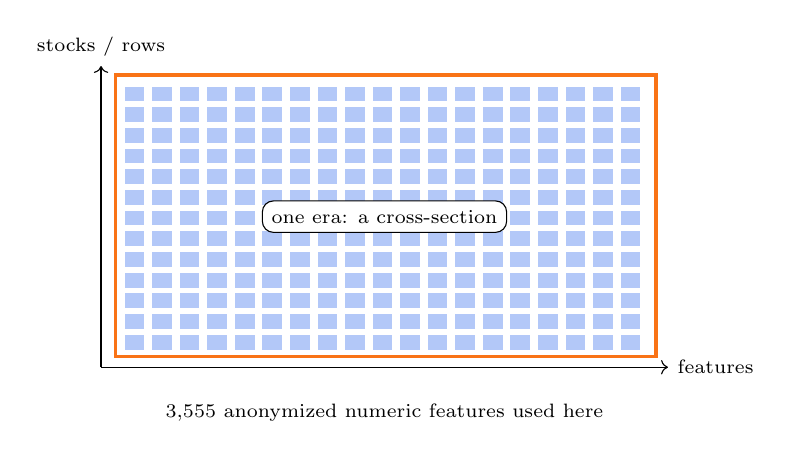
\begin{tikzpicture}[x=1cm,y=.75cm,every node/.style={font=\scriptsize}]
      \draw[->] (0,0)--(7.2,0) node[right]{features};
      \draw[->] (0,0)--(0,5.1) node[above]{stocks / rows};
      \foreach \x in {0.3,0.65,...,6.8} \foreach \y in {.3,.65,...,4.7}
        \fill[blue!35!white] (\x,\y) rectangle +(0.25,0.25);
      \draw[orange,very thick] (0.18,0.18) rectangle (7.05,4.95);
      \node[fill=white,draw,rounded corners] at (3.6,2.55) {one era: a cross-section};
      \node[below] at (3.6,-.45) {3,555 anonymized numeric features used here};
    \end{tikzpicture}
  \column{0.44\textwidth}
    \begin{block}{Rows, eras, target}
      \begin{itemize}
        \item Each row represents one anonymized security at one historical date
        \item An \textbf{era} groups rows from the same market period
        \item Features are anonymized engineered signals; semantics are intentionally hidden
        \item Primary label: Numerai v5.3 main \texttt{target}
        \item Model output is ranked within each era before CORR scoring
      \end{itemize}
    \end{block}
    \small\color{muted}The task is cross-sectional prediction through time—not forecasting one price series.
  \end{columns}
\end{frame}

\begin{frame}{Train / validation / test through time}
  \centering
  \fig{0.94}{figures/chronological-split.png}
  \vspace{-0.3em}
  \begin{columns}[T]
    \column{0.31\textwidth}\centering\textbf{Train}\par Fit weights on earlier eras.
    \column{0.31\textwidth}\centering\textbf{Inner validation}\par Choose architecture and optimizer settings inside training history.
    \column{0.31\textwidth}\centering\textbf{Outer test}\par Evaluate one frozen decision on immediately later eras.
  \end{columns}
  \vspace{0.5em}
  \small\color{muted}In production one would periodically retrain on newly resolved labels. The experiment instead freezes one historical decision so its out-of-time evidence remains interpretable.
\end{frame}

\begin{frame}{What exactly is being optimized?}
  \begin{columns}[c]
  \column{0.51\textwidth}
    \begin{block}{AdamW baseline}
      \[\theta_{t+1}=\theta_t-\eta\,\mathrm{AdamW}(g_t)\]
      Uses the full minibatch gradient, adaptive coordinate scaling and decoupled weight decay.
    \end{block}
    \begin{block}{Spectral wrapper}
      \[C_t=\beta C_{t-1}+(1-\beta)g_tg_t^\top,\quad C_t\in\mathbb{R}^{p\times p}\]
      \[C_tQ_k=Q_k\Lambda_k,\qquad \tilde g_t=(1-\alpha)g_t+\alpha Q_kQ_k^\top g_t\]
      AdamW receives the filtered gradient $\tilde g_t$.
    \end{block}
  \column{0.45\textwidth}
    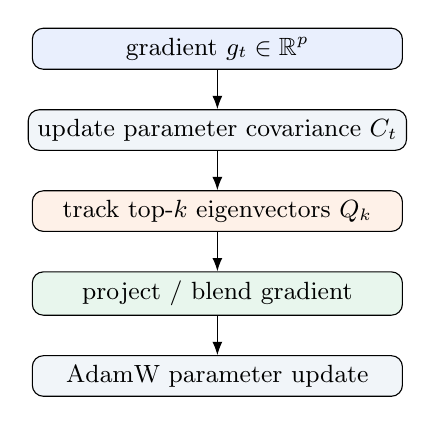
\begin{tikzpicture}[node distance=.5cm,every node/.style={font=\small}]
      \node[draw,rounded corners,fill=blue!10,minimum width=4.7cm] (g) {gradient $g_t\in\mathbb{R}^p$};
      \node[draw,rounded corners,fill=pale,below=of g,minimum width=4.7cm] (c) {update parameter covariance $C_t$};
      \node[draw,rounded corners,fill=orange!10,below=of c,minimum width=4.7cm] (q) {track top-$k$ eigenvectors $Q_k$};
      \node[draw,rounded corners,fill=green!10,below=of q,minimum width=4.7cm] (p) {project / blend gradient};
      \node[draw,rounded corners,fill=pale,below=of p,minimum width=4.7cm] (a) {AdamW parameter update};
      \foreach \x/\y in {g/c,c/q,q/p,p/a} \draw[-{Latex}] (\x)--(\y);
    \end{tikzpicture}
  \end{columns}
\end{frame}

\begin{frame}{The first implementation question mattered}
  \begin{columns}[T]
  \column{0.47\textwidth}
    \begin{block}{Wrong object for the intended optimizer}
      A $B\times B$ batch Gram matrix describes relationships among the $B$ examples currently sampled. Its eigenvectors live in \emph{sample space}.
    \end{block}
    \centering
    $G G^\top\in\mathbb{R}^{B\times B}$\\[0.4em]
    \bad{not the persistent parameter directions requested}
  \column{0.47\textwidth}
    \begin{block}{Correct object tested later}
      A $p\times p$ covariance (implemented with a low-rank basis) tracks directions in the model's parameter space across updates.
    \end{block}
    \centering
    $G^\top G\in\mathbb{R}^{p\times p}$\\[0.4em]
    \good{eigenvectors are parameter directions}
  \end{columns}
  \vspace{0.8em}
  \centering\large The original negative result and the corrected high-rank result are studies of materially different interventions.
\end{frame}

\begin{frame}{The complete research arc}
  \centering
  \fig{0.94}{figures/research-chronology.png}
  \vspace{-0.4em}
  \small\color{muted}Effect sizes are shown to explain direction and chronology; they are not pooled because datasets, capacities, endpoints and protocols differed.
\end{frame}

\begin{frame}{Phase I: corrected low rank still failed}
  \begin{columns}[T]
  \column{0.58\textwidth}
    \fig{1.0}{vendor/exp006-rank-response.png}
  \column{0.38\textwidth}
    \begin{block}{Result}
      \begin{itemize}
        \item Corrected $p\times p$ hard filter
        \item Ranks 1--32, three selection replicas
        \item Rank 16 selected on validation
        \item Five-seed untouched test
        \item AdamW: 0.01686 CORR
        \item Spectral: 0.00061 CORR
        \item \bad{$\Delta=-0.01625$}
      \end{itemize}
    \end{block}
    \small\color{muted}Lesson: correctness alone was insufficient. A tiny rank can discard almost the entire useful update in a multi-million-dimensional model.
  \end{columns}
\end{frame}

\begin{frame}{Phase II: force the model to overfit}
  \begin{columns}[T]
  \column{0.64\textwidth}
    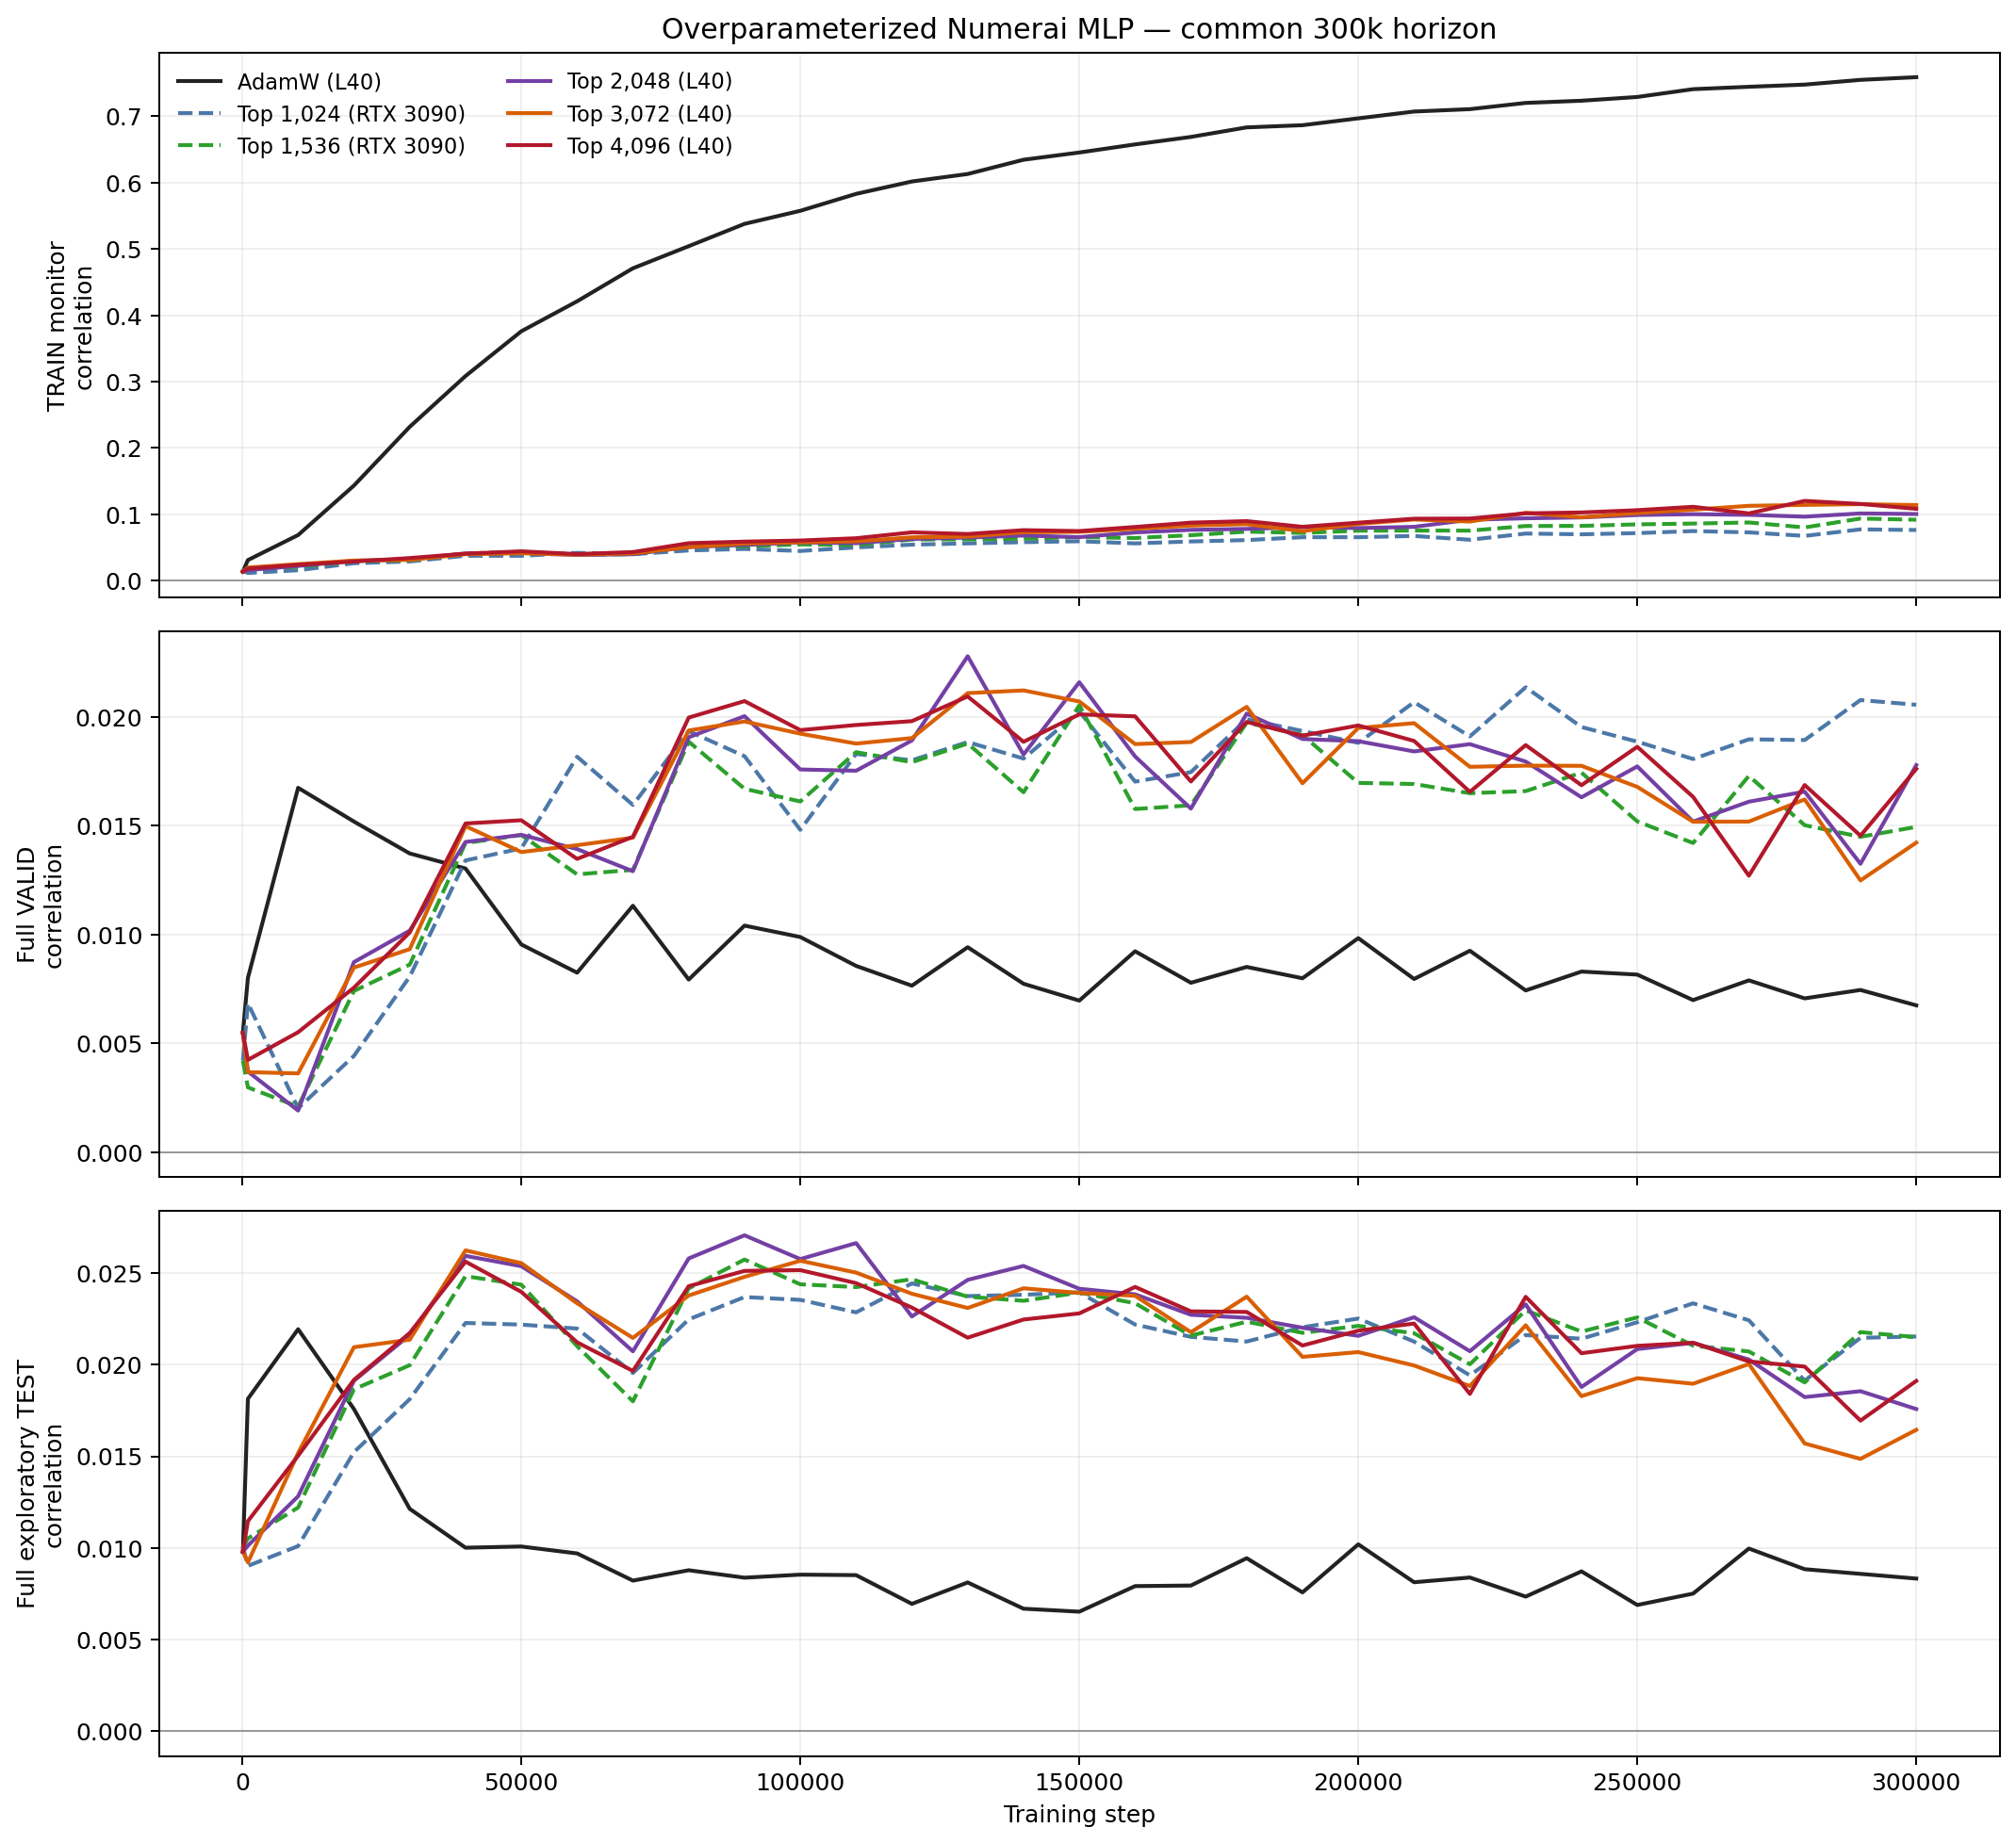
\includegraphics[width=\textwidth,height=0.72\textheight,keepaspectratio]{vendor/exp007-correlation-rank-grid.png}
  \column{0.32\textwidth}
    \small
    \begin{block}{Stress test}
      \begin{itemize}
        \item 13.7M-parameter MLP
        \item Same architecture and batch stream
        \item AdamW vs top-$k$ spectral projection
        \item $k=1{,}024$ to $4{,}096$
        \item Up to one million updates
      \end{itemize}
    \end{block}
    \begin{block}{Observed mechanism}
      AdamW reached 0.76 train CORR while validation deteriorated. Spectral stayed near 0.07--0.11 and retained later-era signal.
    \end{block}
  \end{columns}
\end{frame}

\begin{frame}{High rank changed the answer}
  \centering
  \fig{0.91}{figures/rank-grid-summary.png}
  \vspace{-0.2em}
  \small\color{muted}Exploratory selection used validation trajectories; the displayed TEST trajectory was repeatedly observed and is not an untouched final holdout. Ranks 1,024/1,536 ran on RTX 3090; others on L40.
\end{frame}

\begin{frame}{Requested rank is not realized rank}
  \begin{columns}[T]
  \column{0.62\textwidth}
    \fig{1.0}{vendor/exp007-effective-rank.png}
  \column{0.34\textwidth}
    \begin{block}{Key diagnostic}
      Requested global ranks of 1,024--4,096 produced mean effective ranks of only roughly 5--22 after blockwise eigenspectrum thresholding.
    \end{block}
    \begin{block}{Interpretation}
      Benefits saturated because the useful persistent subspace was much smaller than the nominal capacity. Rank is a ceiling, not necessarily the number of active directions.
    \end{block}
  \end{columns}
\end{frame}

\begin{frame}{Why we did not run the six-week exhaustive plan}
  \begin{columns}[T]
  \column{0.47\textwidth}
    \begin{block}{Original ambition}
      \begin{itemize}
        \item 40 paired configurations
        \item Multiple update budgets
        \item Multiple inner folds and seeds
        \item High-rank amendments
        \item Three nested outer blocks
        \item Sealed validation and live packaging
      \end{itemize}
    \end{block}
  \column{0.47\textwidth}
    \begin{block}{Bounded decision}
      \begin{itemize}
        \item User requested a one-day answer
        \item Runtime cannot select winners
        \item Incomplete F1 results excluded
        \item Complete F0 nominates two IDs
        \item Equal confirmation coverage
        \item One untouched outer block
      \end{itemize}
    \end{block}
  \end{columns}
  \vspace{0.7em}
  \centering\large Goal: decide whether spectral is credible enough to continue—not certify a leaderboard submission.
\end{frame}

\begin{frame}{The bounded protocol}
  \centering
  \fig{0.88}{figures/search-funnel.png}
  \vspace{-0.2em}
  \begin{block}{Leakage controls}
    Candidate nomination used only the complete 5,000-update screen. Both optimizers then ran both IDs 38 and 39 on two inner folds and two seeds. One winner per optimizer was frozen before any outer score existed.
  \end{block}
\end{frame}

\begin{frame}{Why AdamW had 6.8M parameters and spectral had 10.2M}
  \centering
  \fig{0.91}{figures/architecture-comparison.png}
  \vspace{-0.35em}
  \begin{columns}[T]
  \column{0.48\textwidth}
    \textbf{Why it happened:} architecture was treated as a hyperparameter. Each optimizer independently selected the pipeline with highest development CORR from the same paired union.
  \column{0.48\textwidth}
    \textbf{What it answers:} ``Which selected training pipeline is better?'' It does \bad{not} answer ``Does spectral filtering improve this exact MLP?''
  \end{columns}
\end{frame}

\begin{frame}{The selected pipelines were materially different}
  \scriptsize
  \begin{tabular}{>{\bfseries}p{2.6cm}p{4.7cm}p{4.7cm}}
    \toprule
    & AdamW winner: config 38 & Spectral winner: config 39 \\
    \midrule
    Model & 4 layers, width 1,024, ReLU & 3 layers, width 1,536, SiLU \\
    Parameters & 6,799,361 & 10,194,433 \\
    Features & all 3,555 & all 3,555 \\
    Batch & 1,024, era-batched & 2,048, row-batched \\
    Examples & 20.48M & 40.96M \\
    Learning rate & $1.2876\times10^{-4}$, cosine & $2.5188\times10^{-3}$, constant \\
    Regularization & dropout 0.10, small weight decay & dropout 0.02, no weight decay, clip 5 \\
    Spectral filter & none & learned, rank 128, strength 1, decay 0.99 \\
    \bottomrule
  \end{tabular}
  \vspace{0.8em}
  \begin{block}{Fairness verdict}
    Symmetric as a \emph{best-pipeline competition}; asymmetric as a \emph{mechanistic optimizer ablation}. The next experiment must run both optimizers on both frozen architectures in the untouched period.
  \end{block}
\end{frame}

\begin{frame}{Audited outer result}
  \centering
  \fig{0.78}{figures/outer-headline.png}
  \vspace{-0.3em}
  \small 78 later eras $\times$ 359,860 rows per seed; frozen configurations; three seeds; exact standalone Numerai CORR; artifact hashes and metric reproduction audited.
\end{frame}

\begin{frame}{Every random seed favoured spectral}
  \centering
  \fig{0.86}{figures/outer-seeds.png}
  \vspace{-0.3em}
  \small\color{muted}Seed-paired differences: +0.00103, +0.00345, +0.00473. Mean: +0.00307 CORR.
\end{frame}

\begin{frame}{The tradeoff: stronger signal, slightly less uniqueness}
  \centering
  \fig{0.82}{figures/metric-tradeoff.png}
  \vspace{-0.5em}
  \small
  \begin{itemize}
    \item CORR improved by 15.5\% relative; CORR Sharpe improved by 23.1\%.
    \item BMC fell by 0.00058: slightly less contribution beyond Ender60.
    \item Acceptable for standalone prediction, but relevant to Numerai payout and model portfolios.
  \end{itemize}
\end{frame}

\begin{frame}{How certain are we?}
  \centering
  \fig{0.82}{figures/seed-uncertainty.png}
  \vspace{-0.2em}
  \begin{block}{Honest reading}
    Three out of three wins are encouraging. But a seed-level $t$ interval is wide with $n=3$ and crosses zero. An era-block bootstrap and two additional untouched outer blocks are needed for a strong statistical claim.
  \end{block}
\end{frame}

\begin{frame}{Where are we versus the Numerai leaderboard?}
  \centering
  \fig{0.91}{figures/leaderboard-context.png}
  \vspace{-0.35em}
  \small Snapshot: round 1330, 12 Aug 2026, top 1,000 models. Live leaderboard CORR20v2 reputation and our historical v5.3 main-target CORR use different targets, horizons and sampling. The numbers can motivate a submission; they cannot imply a rank.
\end{frame}

\begin{frame}{What competitors get—and why comparison is hard}
  \small
  \begin{tabular}{>{\bfseries}p{3.0cm}rrp{5.0cm}}
    \toprule
    Public metric & median & 90th pct. & maximum / caveat \\
    \midrule
    CORR20v2 reputation & 0.00926 & 0.01466 & 0.01959; live rolling reputation \\
    CORJ60 reputation & 0.01054 & 0.01918 & 0.03262; different neutralized target \\
    BMC reputation & 0.00633 & 0.00967 & 0.01720; contribution relative to benchmark ensemble \\
    MMC reputation & 0.00399 & 0.00658 & 0.01262; contribution relative to metamodel \\
    \midrule
    Our spectral outer CORR & \multicolumn{2}{c}{\textbf{0.02293}} & historical main-target result; not live reputation \\
    Our spectral BMC & \multicolumn{2}{c}{0.00404} & historical Ender60-relative contribution \\
    \bottomrule
  \end{tabular}
  \vspace{0.8em}
  \begin{block}{Only decisive comparison}
    Freeze the procedure, create a resource-valid live callable, submit unstaked for enough rounds, then compare like-for-like live reputations.
  \end{block}
\end{frame}

\begin{frame}{What the result does—and does not—establish}
  \begin{columns}[T]
  \column{0.47\textwidth}
    \begin{block}{Supported}
      \begin{itemize}
        \item Spectral is worth continued investigation
        \item Selected spectral pipeline generalized better on outer block 1
        \item High-rank filtering can arrest MLP memorization
        \item Benefits are rank- and regime-dependent
        \item Runtime disadvantage is irrelevant to this scientific question
      \end{itemize}
    \end{block}
  \column{0.47\textwidth}
    \begin{block}{Not supported yet}
      \begin{itemize}
        \item Spectral filtering alone caused +0.00307
        \item Rank 128 is globally optimal
        \item The gain persists across all historical regimes
        \item The model beats current live competitors
        \item A production submission will have positive payout metrics
      \end{itemize}
    \end{block}
  \end{columns}
\end{frame}

\begin{frame}{The highest-value next experiment}
  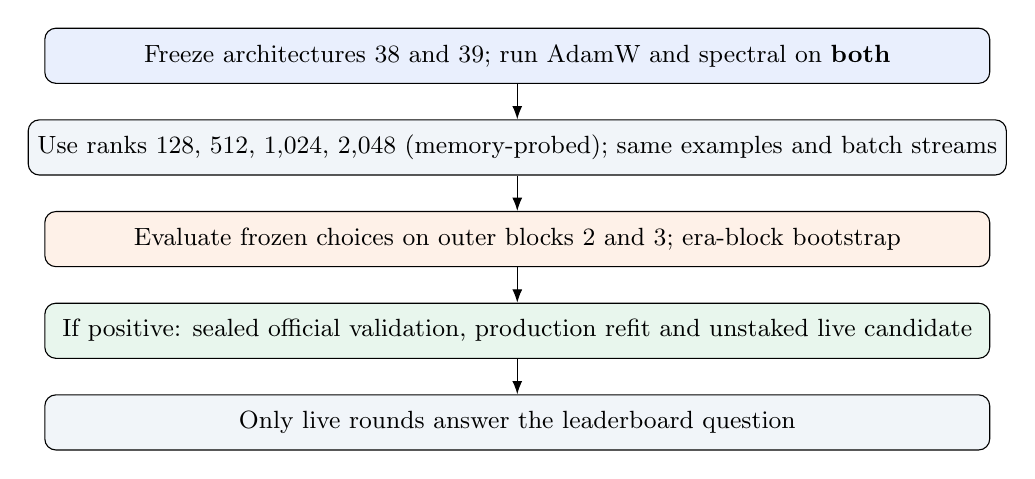
\begin{tikzpicture}[node distance=.45cm,every node/.style={font=\small}]
    \node[draw,rounded corners,fill=blue!10,minimum width=12cm,minimum height=.7cm] (a) {Freeze architectures 38 and 39; run AdamW and spectral on \textbf{both}};
    \node[draw,rounded corners,fill=pale,below=of a,minimum width=12cm,minimum height=.7cm] (b) {Use ranks 128, 512, 1,024, 2,048 (memory-probed); same examples and batch streams};
    \node[draw,rounded corners,fill=orange!10,below=of b,minimum width=12cm,minimum height=.7cm] (c) {Evaluate frozen choices on outer blocks 2 and 3; era-block bootstrap};
    \node[draw,rounded corners,fill=green!10,below=of c,minimum width=12cm,minimum height=.7cm] (d) {If positive: sealed official validation, production refit and unstaked live candidate};
    \node[draw,rounded corners,fill=pale,below=of d,minimum width=12cm,minimum height=.7cm] (e) {Only live rounds answer the leaderboard question};
    \foreach \x/\y in {a/b,b/c,c/d,d/e} \draw[-{Latex}] (\x)--(\y);
  \end{tikzpicture}
  \vspace{0.5em}
  \begin{block}{Go / no-go criterion}
    Continue only if spectral improves exact CORR on both architectures or preserves CORR while materially improving stability/BMC across outer blocks.
  \end{block}
\end{frame}

\begin{frame}{Future work, ordered by information per GPU-hour}
  \small
  \begin{tabular}{clp{7.6cm}}
    \toprule
    Priority & Experiment & Decision unlocked \\
    \midrule
    1 & Matched-architecture $2\times2$ & Separates optimizer effect from model/HPO effect \\
    2 & Outer blocks 2 and 3 & Tests regime robustness and tightens uncertainty \\
    3 & Rank ladder to 2,048+ & Locates saturation under the official-data pipeline \\
    4 & Equal examples / compute diagnostics & Separates more data exposure from filtering \\
    5 & Era-block bootstrap & Quantifies temporal rather than seed-only uncertainty \\
    6 & Sealed official validation & Produces historical score with frozen procedure \\
    7 & Unstaked live submission & Establishes actual leaderboard comparability \\
    8 & Continual retraining simulation & Approximates the real finance deployment loop \\
    \bottomrule
  \end{tabular}
\end{frame}

\begin{frame}{Bottom line}
  \begin{columns}[c]
  \column{0.58\textwidth}
    \fig{1.0}{figures/outer-headline.png}
  \column{0.38\textwidth}
    {\Large\bfseries\color{green}The spectral idea survived the go/no-go test.}\par
    \vspace{0.8em}
    It won all three frozen outer seeds and improved both average CORR and stability.\par
    \vspace{0.8em}
    {\color{orange}\bfseries But the selected pipelines differed in architecture, batch size and examples seen.}\par
    \vspace{0.8em}
    The result justifies one controlled follow-up—not a leaderboard claim.
  \end{columns}
\end{frame}

\appendix

\begin{frame}{Appendix: why the original theoretical story weakened}
  \small
  For scalar-output losses, a per-example gradient often factors as
  \[g_i = \ell_i'(f_\theta(x_i),y_i)\,\nabla_\theta f_\theta(x_i).\]
  Normalizing $g_i$ can remove the residual magnitude and leave mainly a sign times the model Jacobian direction. In the original $B\times B$ construction, target permutation therefore changes signs but can preserve the eigenspectrum. ``Gradient consensus'' may measure shared Jacobian / feature structure rather than target signal.
  \vspace{0.7em}
  \begin{block}{Why the current result can still be real}
    The corrected learned $p\times p$ filter acts as a history-dependent optimizer regularizer. It may suppress rapidly changing parameter directions even if the original label-consensus interpretation is incomplete.
  \end{block}
\end{frame}

\begin{frame}{Appendix: audit trail}
  \tiny
  \begin{tabular}{>{\bfseries}p{3.3cm}p{8.4cm}}
    \toprule
    Artifact & Role \\
    \midrule
    \texttt{selection-one-day-}\newline\texttt{f0-top1.json} & Frozen F0 nominations from complete equal-coverage screen \\
    \texttt{selection-one-day-}\newline\texttt{confirmed-top1.json} & Development-only winners and score-file hashes \\
    \texttt{submission-one-day-}\newline\texttt{outer1.tsv} & Exact six-cell frozen outer manifest \\
    \texttt{outer-results.csv} & Six metrics rows with signatures and artifact hashes \\
    \texttt{outer-audit.json} & Split, seeds, selected IDs, rows and manifest hash \\
    commit \texttt{7dac4cd} & Allows sub-ppm float32 serialization roundoff while retaining metric-reproduction checks \\
    \bottomrule
  \end{tabular}
  \vspace{0.6em}
  \par\raggedright
  The audit reproduced metrics from stored predictions, verified all 78 expected outer eras, checked row uniqueness/alignment, configuration provenance, model signatures, and prediction/result SHA-256 hashes.
\end{frame}

\begin{frame}{Appendix: evidence map}
  \small
  \begin{tabular}{>{\bfseries}p{2.2cm}p{3.0cm}p{3.1cm}p{4.5cm}}
    \toprule
    Phase & Question & Outcome & Main limitation \\
    \midrule
    exp-001--005 & Does original $B\times B$ filter transfer? & Negative; target-independence insight & Different intervention from intended $p\times p$ optimizer \\
    exp-006 & Does corrected low-rank hard projection work? & No; rank 16 severely harmed CORR & Tiny rank, small model, limited tuning \\
    exp-007 & Can high rank prevent memorization? & Yes, strongly in overparameterized MLP & Exploratory TEST trajectory; one seed \\
    exp-008 & Is selected spectral pipeline a serious competitor? & Yes: +0.00307 outer CORR, 3/3 seeds & Different selected architectures; one outer block \\
    \bottomrule
  \end{tabular}
\end{frame}

\begin{frame}[plain]
  \vfill
  \centering
  {\Huge\bfseries Questions?}\par
  \vspace{1em}
  {\large\color{muted}Recommended next step: matched-architecture outer evaluation before sealed validation.}
  \vfill
\end{frame}

\end{document}
